%!TEX TS-program = xelatex
%!TEX encoding = UTF-8 Unicode

\documentclass[11pt,tikz,border=1]{standalone}
\usetikzlibrary{positioning,decorations.pathreplacing}

\begin{document}
  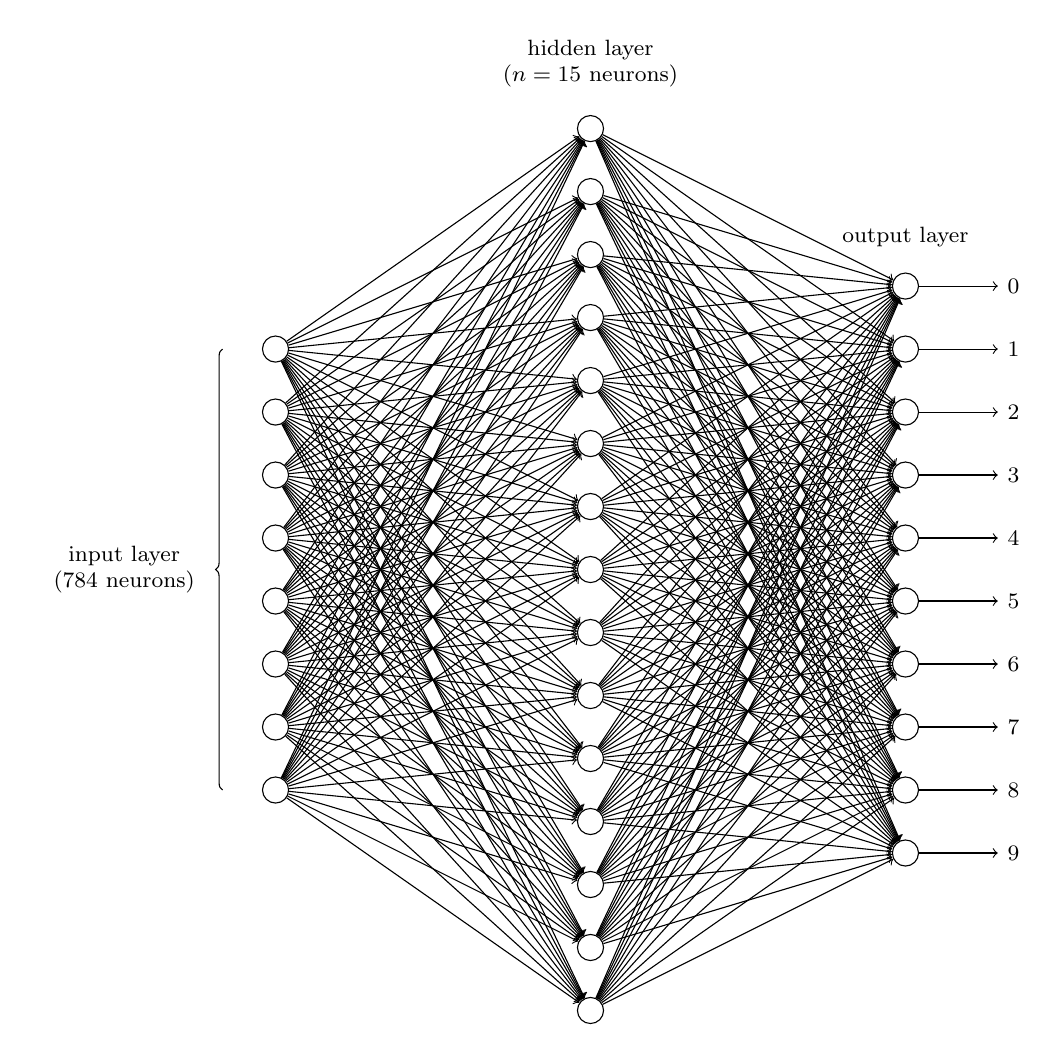
\begin{tikzpicture}[
    neuron/.style={circle,draw,inner sep=0pt,minimum size=5mm},
    font=\footnotesize
    ]

    % leftmost layer:
    \foreach \y in {1,...,8}
    \node (l\y) at (-4, 7.5 / 1.25 - 4 / 1.25 + \y / 1.25) [circle,draw] {};

    % hidden layer:
    \foreach \y in {1,...,15}
    \node (m\y) at (0, \y / 1.25) [circle,draw] {};

    % output layer:
    \foreach \y in {1,...,10}
    \node (r\y) at (4, 7.5 / 1.25 - 5 / 1.25 + \y / 1.25) [circle,draw] {};

    \foreach \y in {1,...,10}
    \node (o\y) [right=of r\y] {$\number \numexpr 10 -\y \relax$};

    \begin{scope}[node distance=2mm]
      \node (text1) [above=of m15] {
        \begin{tabular}{c}
          hidden layer \\
          ($n = 15$ neurons)
    	\end{tabular}
      };
      \node (text2) [above=of r10] {
        output layer
      };
    \end{scope}

    % draw brace:
    \draw[decorate,decoration={brace,mirror}] ([xshift=-5mm]l8.west) -- ([xshift=-5mm]l1.west) node [midway,xshift=-12.5mm] {
      \begin{tabular}{c}
        input layer \\
        ($784$ neurons)
      \end{tabular}
    };

    % connections:
    \foreach \x in {1,...,8}
    \foreach \y in {1,...,15}
    \draw [->] (l\x) to (m\y);

    \foreach \x in {1,...,15}
    \foreach \y in {1,...,10}
    \draw [->] (m\x) to (r\y);

    \foreach \x in {1,...,10}
    \draw [->] (r\x) to (o\x); 

  \end{tikzpicture} 
\end{document}
